\chapter{Desenvolvimento}

A metodologia será baseada no método \emph{Scrum, ``método ágil utilizado para a gestão e desenvolvimento de projetos que têm um curto prazo de entrega.''}.[25] Este método foi aplicado ao coletar os pontos positivos e negativos do grupo e definir os papeis de cada colaborador, considerando o nível de complexidade do projeto e o tempo disponível para sua elaboração.

As etapas do desenvolvimento do projeto descritas na Figura \ref{fig:etapas_dev} apresentam os parâmetros iniciais, escolha dos materiais e simulação. 

\begin{figure}[ht!]
\centering
\caption{Etapas de desenvolvimento}
\label{fig:etapas_dev}
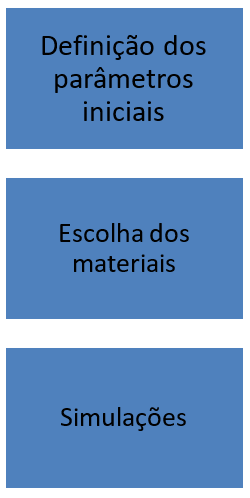
\includegraphics{etapas_dev}
\smallcaption{Fonte: Autor}
\end{figure}

\section{Parâmetros iniciais de projeto}

Os parâmetros iniciais de projeto foram determinados a partir das referências coletadas em artigos científicos e produtos disponíveis no mercado.

\begin{itemize}
	\item \mbox{$P_out$} = 5 W
	\item Distância de transmissão = 5 metros
	\item Eficiência > 50\%
\end{itemize}

\section{Sistema}

O sistema de transferência de energia a laser, foi elaborado baseando-se no sistema DLC [26].

No ganho médio os retrorrefletores permitem refletir fótons na mesma direção, mas com sentido aposto e com uma pequena defasagem. No retorno, os fótons passam pelo ganho médio onde o feixe é formado e é refletido novamente. O retrorrefletor no receptor permite que parte da energia do laser chegue na célula solar. Essa abordagem faz com que qualquer obstáculo entre o transmissor e o receptor, interrompa o laser, pois os fótons não voltam para formar o laser no ganho médio.

\subsection{Laser}

Para a seleção do laser, foram considerados os parâmetros:

\subsubsection{Possibilidade para transferir energia através da atmosfera}

A fim de maximizar a eficiência na transferência de energia, os lasers devem operar em uma faixa de energia em que as placas fotovoltaicas possam ser mais otimizadas. A janela na região entre 780 e 1100 nm é particularmente relevante para a tecnologia de transmissão de energia sem fio.

\subsubsection{Possibilidade para transferir a energia o maior tempo possível}

O feixe do laser deve ser brilhante o suficiente para garantir que a energia possa ser transferida em um longo intervalo de tempo. O fluxo $\Phi$ entregue ao receptor na faixa inclinada $L$ é dado pela equação.

\begin{equation}
\label{eq:gaussiano}
\Phi = \frac{R_{source} A_{source} \eta_{trans}}{L^2}
\end{equation}

Onde $R_{source}$ é a radiância (potência por unidade de área) da fonte do laser, uma constante que indica a qualidade do feixe e não pode ser alterada por ótica passiva; $A_{source}$ é a área total da fonte do feixe, $L$ é o alcance de transmissão e  $\eta_{trans}$ é a eficiência de transmissão através da atmosfera.

\subsubsection{Laser Diodo}

O laser diodo trabalhando no modo pulso, é a melhor opção para esse tipo de projeto, pois é o que apresenta melhor eficiência, confiabilidade e menor tamanho em relação aos outros tipos disponíveis no mercado [27].

A corrente injetada tem influência direta na eficiência de conversão que gira em torno de 50\% [27].

Para uma análise preliminar foram selecionados componentes que apresentam potência de saída maior que a requerida do projeto, Figura \ref{fig:modelo_1} e Figura \ref{fig:modelo_2}. Além disso, o tamanho também foi um dos pontos importantes para a seleção, sendo $I_{SE}$ é o índice \emph{Slope Efficiency}, \mbox{$P_{out_min}$} potência mínima de saída, \mbox{$E_{min}$} eficiência mínima e \mbox{$\lambda$} é o comprimento de onda, Tabela \ref{tab:comp_modelo}.

\begin{table}[ht!]
	\caption{Comparativo dos modelos selecionados}
	\label{tab:comp_modelo}
	\begin{tabular}{c|c|c|c|c|c}
		\hline
		\textbf{Laser} & \textbf{Modelo} & \textbf{\mbox{$P_{out_{min}}$} (W)} & \textbf{\mbox{$I_{SE}$} (W/A)} & \textbf{\mbox{$E_{min}$} (\%)} & \textbf{\mbox{$\lambda$} (nm)}\\
		\hline
		Laser 1 & RLS/LD-808NM-15W & 15 & 1,8 & 40 & 808\\
		\hline
		Laser 2 & K808DAECN-25.00W & 25 & 4 & 40 & 808\\
		\hline
		Laser 3 & RL915NM-10W & 10 & - & 40 & 915\\
		\hline
	\end{tabular}
	\smallcaption{Fonte: Adaptado de \url{http://pelicano.ipen.br/PosG30/TextoCompleto/Martha\%20Simoes\%20Ribeiro_D.pdf}. Acessado em: 22/05/2021}
\end{table}

\begin{figure}[ht!]
\centering
\caption{Optica do feixe}
\label{fig:modelo_1}
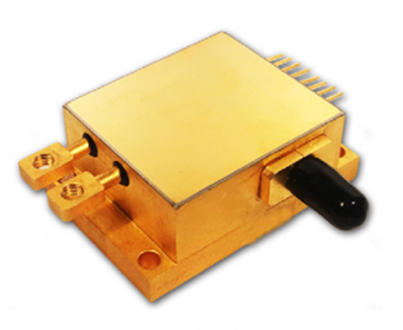
\includegraphics{modelo_1}
\smallcaption{Fonte: Laser Diode Source. Disponível em: \url{https://www.laserdiodesource.com/files/pdfs/laserdiodesource_com/4776/808nm_25W_Detachable_Fiber_Diode_Laser_BWT-1609445237.pdf}. Acesso em: 30 maio 2021.}
\end{figure}

\begin{figure}[ht!]
\centering
\caption{Optica do feixe}
\label{fig:modelo_2}
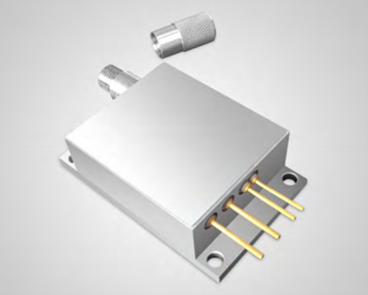
\includegraphics{modelo_2}
\smallcaption{Fonte: Laser Diode Source. Disponível em: \url{https://www.laserdiodesource.com/files/pdfs/laserdiodesource_com/4776/808nm_25W_Detachable_Fiber_Diode_Laser_BWT-1609445237.pdf}. Acesso em: 30 maio 2021.}
\end{figure}

\subsection{Painel Fotovoltaico}

Nas células fotovoltaicas, para gerar eletricidade, os fótons devem ter energia maior ou igual ao intervalo de banda do material. Uma vez que a energia de um fóton é proporcional à sua frequência, as células PV respondem a determinadas frequências de luz correspondentes ao intervalo de banda da célula energética.

Os principais fatores a serem considerados para que a potência possa ser efetivamente convertida em eletricidade são:

\begin{itemize}
	\item Potência do laser;
	\item Comprimento de onda;
	\item Temperatura;
	\item Material das células
\end{itemize}

As curvas de resposta espectral para alguns materiais de PV diferentes são ilustradas na Figura \ref{fig:resposta_espectral}.

\begin{figure}[ht!]
\centering
\caption{Resposta espectral}
\label{fig:resposta_espectral}
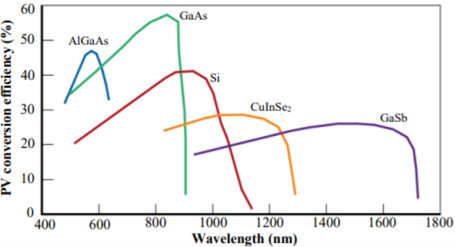
\includegraphics{resposta_espectral}
\smallcaption{Fonte: JIN, Ke; ZHOU, Weiyang. Wireless Laser Power Transmission: a review of recent progress. Ieee Transactions On Power Electronics, [s. l], v. 34, n. 4, p. 3842-3859, 05 jul. 2018. Disponível em: \url{https://ieeexplore.ieee.org/document/8404085}. Acesso em: 09 maio 2021.}
\end{figure}

Percebe-se que a célula fotovoltaica de Arseneto de Gálio (GaAs) apresenta uma melhor eficiência em relação ao comprimento de onda entre 800nm e 850nm. Porém, seu alto custo o torna inviável para utilização. Portanto, as células de Silício (Si) que apresentam uma melhor aplicação entre 850 nm e 1064 nm serão as utilizadas no projeto.